\documentclass[preview]{standalone}
\usepackage{pgfplots}
\usepackage{amsmath}

\begin{document}
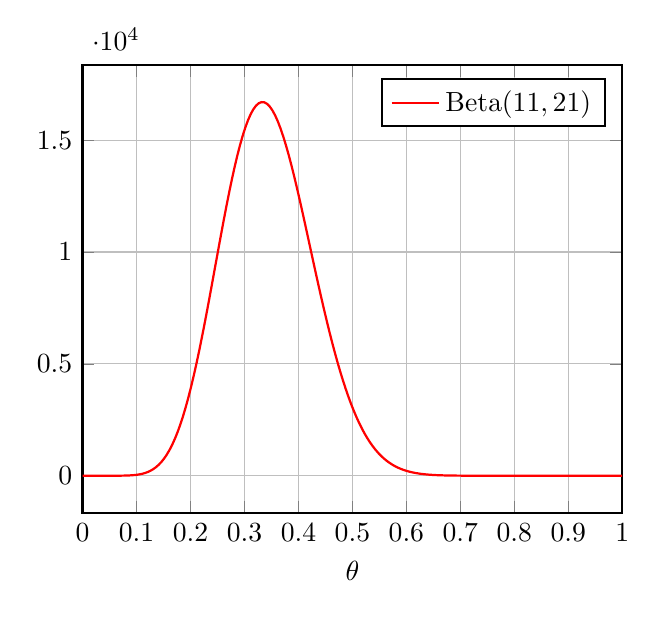
\begin{tikzpicture}
    \begin{axis}[
        domain=0:1,
        samples=200,
        thick,
        legend pos=north east,
        xlabel={$\theta$},
        grid=major,
        xmin=0, xmax=1,
        xtick={0,0.1,...,1},
    ]
        % Beta(11,22) -> B(11,22) ≈ 
        \addplot[red] {3.28e+12 * x^(11-1) * (1-x)^(21-1)};
        \addlegendentry{$\text{Beta}(11,21)$}
    \end{axis}
\end{tikzpicture}
\end{document}
